\chapter{Смешение волн на $\Delta$-системе}
Как упоминалось ранее, долгое время исследования в экспериментальной квантовой оптике были сосредоточены на изучении ансамблей природных, или естественных атомов \cite{Miller_2005,Walther_2006}. Однако, сверхпроводящие искусственные атомы крайне привлекательны для изучения явлений квантовой оптики. Их энергетические уровни могут быть спроектированы со значительным отличием от естественных атомов, и сильная связь с полем достигается не только в высокодобротных резонаторах \cite{wallraff2004strong}, но и в линих передачи (волноводах) \cite{Astafiev2010resonance, vanLoo1494}. Это позволяет воспроизводить явления квантовой оптики и даже достигать режимов, недоступных для естественных атомов. Интерес для применений представляют такие явления, как когерентный захват заселенности, электромагнитно-индуцированная прозрачность, расщепление Аутлера-Таунса --- многие из них были представлены в разделе \ref{sec: microwave qo}. В данной работе представлены также результаты по непрерывному волновому смешению (Глава \ref{ch: cwm}) и квантовому волновому смешению (Глава \ref{ch: q_mixing}), которые были впервые экспериментально изучены в сверхпроводящих искусственных атомах. Кроме того, сверхпроводящие трехуровневые системы могут быть использованы для охлаждения квантовых систем, усиления микроволновых сигналов и генерации одиночных или запутанных пар фотонов --- всего того, что является важным для создания квантовых сетей \cite{kimble2008quantum}.

В данной главе представлены результаты эксперимента по трехволновому квантовому смешению \cite{liu2014controllable}. Это нелинейный эффект, который может возникать в циклических трехуровневых атомах, фактически отсутствующих в природе, но легко реализуемых с помощью сверхпроводящих искусственных атомов. Единственными подходящими естественными системами для трехволнового смешения являются хиральные молекулярные трехуровневые системы без инверсионной симметрии \cite{PhysRevLett.111.023008}. Однако эти системы не могут быть перестраиваемыми по частоте. В отличие от параметрических трехволновых смесительных устройств на основе джозефсоновского перехода, которые полагаются на смешивание по классической нелинейности, мы реализуем здесь другой метод генерации трехволнового смешивания с использованием одного искусственного атома циклического типа, или $\Delta$-типа. Мы непосредственно измеряем когерентное излучение циклического трехуровневого атома при двух внешних резонансных возбуждающих сигналах, соответствующих двум атомным переходам \cite{PhysRevA.98.041801}. Помимо частот накачки, излучение происходит еще на одной частоте --- сумме или разности частот драйва. Это излучение является следствием когерентного преобразования частоты, но по своей сути отличается от классического нелинейного преобразования частоты, которое привело бы к появлению боковых компонент на суммарной и разностной частотах. Ранее когерентные атомные возбуждения с использованием двух частот были исследованы при помощи фазового кубита, являющегося квантовой системой с двумя внутренними степенями свободы \cite{Lecocq2012}. Однако, состояние фазового кубита измерялось с помощью тока переключения, в то время как прямое детектирование когерентно преобразованного сигнала на циклическом искусственном атоме в открытом пространстве дает некоторые преимущества. В частности, можно непосредственно использовать когерентную (упругую) составляющую излучаемого поля на суммарной или разностной частоте переходов искусственного атома. Это открывает путь к инновационной квантовой электронике на основе трехволнового смешения или когерентного преобразования частоты.
\section{Режим $\Delta$-системы в потоковом кубите}
\begin{figure}
	\centering
	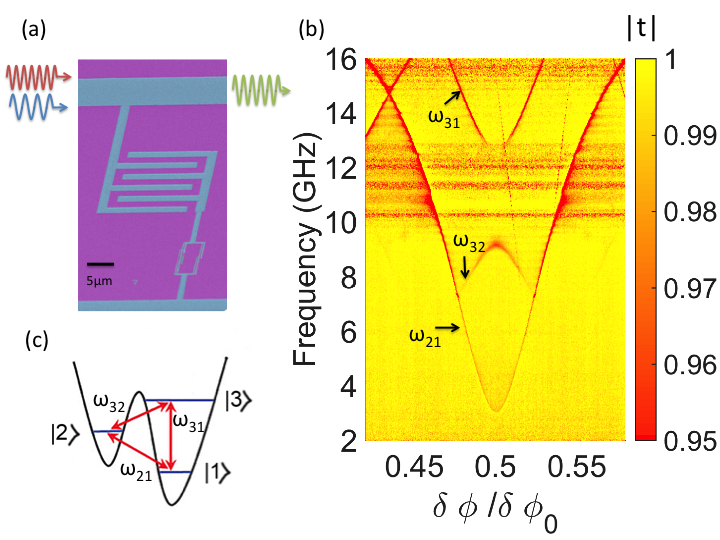
\includegraphics[width=0.8\textwidth]{figure1_Delta.png}
	\caption[Потоковый кубит в режиме $\Delta$-системы]{Сильно связанный с волноводом потоковый кубит, состоящий из 4 джозефсоновских переходов, электронное изображение которого представлено на панели (a), может находиться в режиме $\Delta$-системы при $\delta\phi \ne 0.5$. Однотоновая спектроскопия представлена на графике (b), верхние переходы становятся видимыми из-за большой мощности тона. (с), принципиальная схема переходов в циклическом атоме. Измерения проводятся при $\omega_{21}/2\pi = 6.48$ ГГц, $\omega_{32}/2\pi = 8.35$ ГГц, и $\omega_{31}/2\pi = 14.83$ ГГц.}
	\label{fig: flux_delta}
\end{figure}
Изучаемое устройство представляет собой потоковый кубит --- сверхпроводниковую петлю площадью около $\sim 10$~мкм$^{2}$, в которую вставлены четыре джозефсоновских перехода. Эта геометрия является модифицированной версией оригинального потокового кубита, предложенного в работе \cite{mooij1999josephson}, где один из трех переходов --- $\alpha$-переход --- имеет в $\alpha$ раз отличную площадь по сравнению с остальными переходами. Один из электродов получившейся петли связан с одномерным волноводом через встречно-штыревую емкость $C=6$~фФ, см. Рис.~\ref{fig: flux_delta}(a). Эта емкость определяет константу релаксации кубита в диапазоне от нескольких МГц до нескольких десятков МГц, в зависимости от частоты кубита. Основные параметры устройства --- джозефсоновская энергия $E_{J}/h=65$~ГГц, зарядовая энергия $E_{C}=e^2/2C$, $E_{C}/h=19$~ГГц и параметр $\alpha=0.45$ --- подобраны таким образом, чтобы все три частоты нижних переходов атома, см. Рис.~\ref{fig: flux_delta}c), попадали в допустимый частотный диапазон 2-18 ГГц нашего высокочастотного измерительного тракта. Скорость излучения в волновод для каждого из этих переходов достаточно велика для того, чтобы безызлучательная релаксация не играла значительной роли для наблюдаемых нами явлений. 

Точные значения частот переходов $\omega_{12}$, $\omega_{23}$, и $\omega_{13}$ контролируются при помощи внешнего магнитного потока, пронизывающего петлю кубита, $\Phi=\Phi_{0}/2+\delta\Phi$, где $\Phi_{0}$ --- квант магнитного потока и $\delta\Phi$ --- отстройка по потоку от точки симметрии, которая соответствует половине кванта магнитного потока. Частоты атомных переходов экспериментально определяются при помощи однотоновой спектроскопии на пропускание, измеряемой при помощи ВАЦ. Мы сканируем частоту пробного сигнала при различных значениях $\delta\Phi$, в результате получая спектр на Рис.~\ref{fig: flux_delta}b). Чтобы увидеть переход $|3\rangle \rightleftarrows |2\rangle$, необходимо значительно поднять мощность микроволнового тона, чтобы вызвать заметную заселенность уровня $\ket{2}$, который практически не заселяется в пределе слабой мощности. 
В рабочей точке по магнитному потоку частоты разрешенных переходов составляют $\omega_{21}/2\pi = 6.48$ ГГц, $\omega_{32}/2\pi = 8.35$ ГГц, и $\omega_{31}/2\pi = 14.83$ ГГц ($\omega_{31} = \omega_{21}+\omega_{32}$),  как схематично показано на Рис.~\ref{fig: flux_delta}(c). Отметим, что все три вышеперечисленные перехода разрешены только при ненулевой отстройке от $\delta\Phi = \Phi_0/2$, в то время как в точке симметрии переход $\ket{1}\rightleftarrows\ket{3}$ является запрещенным из соображений симметрии. Все измерения проводятся при базовой температуре криостата 12-15 мК, при которой тепловая заселенность пренебрежимо мала и не оказывает влияния на ход эксперимента.

\section{Описание эксперимента}
После завершения начальной характеризации образца, мы подаем на $\Delta$-систему два непрерывных сигнала, частоты которых практически совпадают с резонансными частотами каких-либо двух атомных переходов, и изучаем когерентное излучение системы на частоте третьего перехода, не возбуждаемого внешними сигналами. 
Измерения в каждом из показанных на Рис.~\ref{fig: 3wm_regimes} режимов проводились при различных значениях амплитуд Раби внешнего поля $\Omega_{ij}$ между состояниями $\ket{i}, \ket{j}$, где $i$ и $j$ принимают значения 1,2,3. Согласно квантовомеханическому описанию, излучение на боковой компоненте может возникнуть только в том случае, если она попадает в резонанс с каким-либо атомным переходом.

\begin{figure}[!th]
	\centering
	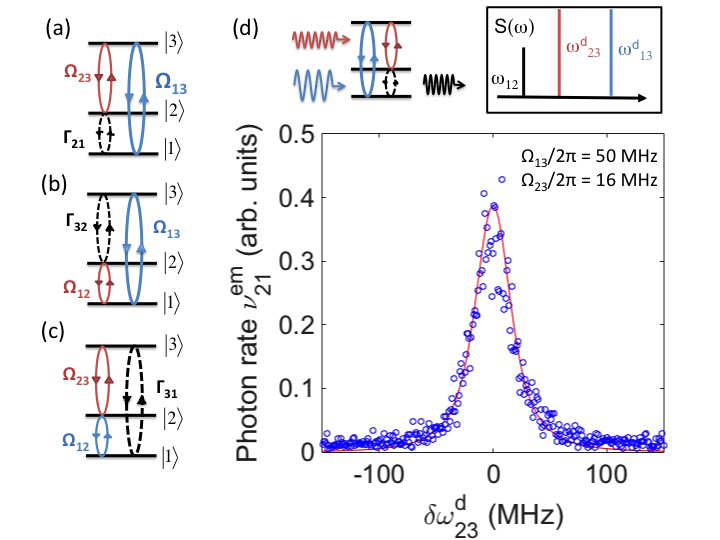
\includegraphics[width=0.8\textwidth]{figure2_Delta.png}
	\caption[Режимы трехволнового смешения на трехуровневой $\Delta$-системе]{Когерентное излучение на трехуровневой системе. Атом накачивается гармоническими сигналами на частотах: (a) $\omega_{23}$ и $\omega_{13}$; (b) $\omega_{12}$ и $\omega_{13}$; (c) $\omega_{12}$ и $\omega_{23}$. Амплитуды полей обозначены как $\Omega$ с индексами, соответствующими номерам уровней. (d) Мощность пика когерентного излучения на частоте $\omega_{12}$ в зависимости от отстройки $\delta\omega_{23}$, выраженная в единицах потока фотонов $\nu_{21}^{\text{em}}$. Атом находится под действием сигналов с амплитудами $\Omega_{23}/2\pi=16$ МГц, $\Omega_{13}/2\pi=50$ МГц. Вставка в правом верхнем углу схематично отражает полный спектр излучения $\Delta$-системы. }
	\label{fig: 3wm_regimes}
\end{figure}

Чтобы понять механизм происходящих физических процессов, можно обратиться к формализму вторичного квантования. При взаимодействия двух когерентных волн с одиночной квантовой системой, только один акт рассеяния (однофотонного или многофотонного) может происходить одномоментно, так как испущенное излучение улетает в волновод, и каскадные процессы становятся невозможными. Введем операторы рождения и уничтожения фотона  $a^{\dagger}_{ij} \text{ и }a_{ij}$ на частоте $\omega_{ij}$, тогда разрешенные многофотонные процессы, ограниченные атомными переходами, описываются членами $a_{31}a_{32}^{\dagger}a_{21}^{\dagger}$ и $a_{31}^{\dagger}a_{32}a_{21}$. Эти два процесса сохраняют полную энергию и объясняют создание фотонов на дополнительных частотах, изображенных на Рис.~\ref{fig: 3wm_regimes}(a-c) пунтктирными линиями.

Сосредоточимся на случае, когда переходы $\ket{1} \rightleftarrows \ket{3}$ и $\ket{2} \rightleftarrows \ket{3}$ возбуждаются близкими к резонансу полями на частотах $\omega_{31}^{d}=\omega_{31}+\delta\omega_{31}$ и $\omega_{32}^{d}=\omega_{32}+\delta\omega_{32}$, при этом измеряется поле на частоте перехода $\ket{2}\rightarrow\ket{1}$. Описываемую систему можно изучать в полуклассическом приближении, где внешние поля связывают атомные состояния через дипольное взаимодействие $\hbar\Omega_{ij}=\phi_{ij}V_{ij}$, где $\phi_{ij}$ --- электрический дипольный момент соответствующего перехода. Дополнительно применяя приближение вращающейся волны, Гамильтониан записываем следующим образом:
\begin{equation}
	\begin{aligned}
		H={}&-\hbar(\delta\omega_{31}\sigma_{11}+\delta\omega_{23}\sigma_{22})\\
		&-\hbar\left[\frac{\Omega_{13}}{2}(\sigma_{13}+\sigma_{31})+\frac{\Omega_{23}}{2}(\sigma_{32}+\sigma_{23})\right],
	\end{aligned}
	\label{H1}
\end{equation}
где $\sigma_{ij}=\ket{i}\bra{j}$. Динамика и стационарное состояние системы с таким гамильтонианом можно определить при помощи основного квантового уравнения, см. раздел \ref{sec:Lind}.

Атом, который взаимодействует с одномерным волноводом, излучает когерентное поле:
\begin{equation}
	V^{em}_{ji}(x,t)=i\frac{\hbar\Gamma_{ji}}{\phi_{ji}}\braket{\sigma_{ij}}e^{i (k_{ji}|x|-\omega_{ji}t)},
	\label{eq:V}
\end{equation}
где $\braket{\sigma_{ij}}=\rho_{ji}$ определяется из стационарного ($\dot{\rho}=0$) решения основного квантового уравнения. Спектральная плотность может быть рассчитана как $S(\omega) = (2\pi)^{-1}\int_{-\infty}^{+\infty}\langle\hat{V}^{em}_{ij}(0)\hat{V}_{ji}^{em}(\tau)\rangle_{ss}e^{i\omega \tau} d\tau$, где индекс ss означает взятие корреллятора по стационарному состоянию. Как пояснялось в разделе \ref{sec: scatt} для двухуровневой системы, эта спектральная плотность состоит из эластичной и неэластичной части. При помощи СА мы измеряем узкий пик, соответствующий эластичной части $S_{coh}=\hbar \omega Z_{0} \Gamma_{ji} \braket{\sigma_{ij}}_{ss} \braket{\sigma_{ji}}_{ss} \delta(\omega-\omega_{ij})$, где введено стандартное обозначение для скорости излучательной релаксации $\Gamma_{ji} = \omega Z_{0}/\hbar \phi_{ji}$. Мощность, сосредоточенная в этом пике, выражается как:
\begin{equation}
	P(\omega)=\frac{\hbar\omega\Gamma_{ji}}{2} |\braket{\sigma_{ij}}|^2,
\end{equation}
где $P=\frac{|V_{ji}^{em}|^2}{2Z_0}$. Частота $\omega$ находится вблизи от частоты перехода $\omega_{21}/ 2\pi=6.48$ ГГц как схематично показано на Рис.~\ref{fig: 3wm_regimes}(d). Эта мощность может измеряться не только при помощи спектрального анализатора, но и любым другим эквивалетным прибором или комбинацией приборов. Далее мы используем термин <<когерентное излучение>> для обозначения амплитуды напряжения $V^{em}$, которую можно однозначно определить из $P(\omega)$. Ширина пика этого излучения определяется шириной спектра генератора, который используется для возбуждения искусственного атома, что и подтверждает когерентность. Мы не проводим специального измерения фазы, но ожидаем что она однозначно связана с суммарной либо разностной фазой накачки, как это подверждается в симуляциях. %We explain simulations later

Общее аналитическое решения для генерируемого в стационарном состоянии поля крайне объемно. В приближении слабого драйва, решение упрощается к выражению: $\langle\sigma_{ij}\rangle\approx\frac{\Omega_{ik}}{\lambda_{ik}}\frac{\Omega_{kj}}{\lambda_{kj}}$, где $\lambda_{mn}=\gamma_{mn}-i\delta\omega_{mn}$ (индексы принимают значения 1,2 или 3). Однако, для эффективной генерации смешанной волны атом должен находиться в режиме сильного возбуждения: $\Omega_{mn}\gg\gamma_{mn}$, где $\gamma_{mn}$ --- полная дефазировка перехода $\ket{m}\rightleftarrows\ket{n}$. Если использовать атом в качестве однокомпонентного смесителя, то максимальная мощность, которую он сможет обеспечить, ограничивается временем релаксации перехода и должна быть $\leq\hbar\omega\Gamma_{ij}/8$, поскольку $|\langle\sigma_{ji}\rangle| \leq 1/2$. Из-за принципа работы, рабочая полоса такого устройства ограничена частотами переходов используемого циклического атома.
\begin{figure}[!htb]
\centering
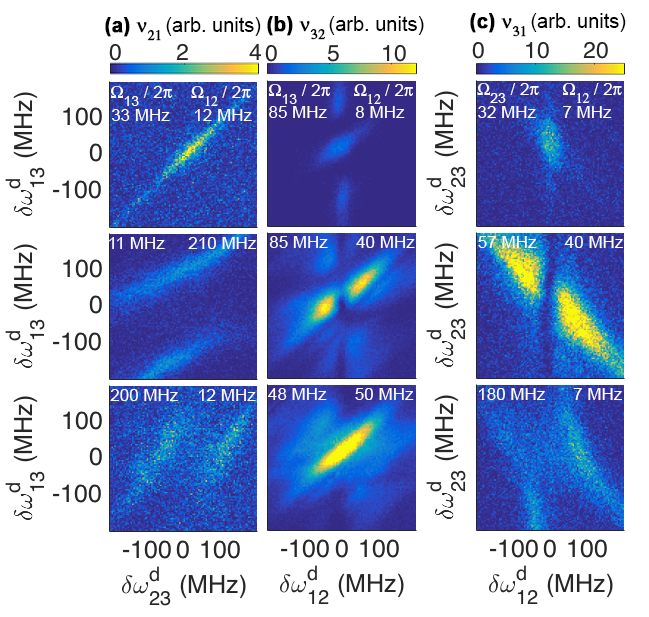
\includegraphics[width=0.85\columnwidth]{fig3_delta.png} 
\caption{Поток фотонов в когерентном излучении  $\nu^{em}$ (относительные единицы) как функция частотной отстройки $\delta\omega^{d}$ какдого из двух возбуждающих сигналов с амплитудами $\Omega_{ij}$. (a) Излучаемый поток фотонов при переходе $\ket{2}\rightarrow \ket{1}$, $\nu^{em}_{21}$ при отмеченных значениях амплитуд $\Omega_{13}$, $\Omega_{23}$. (b) Излучаемый поток фотонов от перехода $\ket{3}\rightarrow \ket{2}$, $\nu^{em}_{32}$, при амплитудах внешних полей $\Omega_{13}$, $\Omega_{12}$. (c): Излучаемый поток фотонов вблизи перехода $\ket{3}\rightarrow \ket{1}$, $\nu^{em}_{31}$, при амплитудах Раби внешних полей $\Omega_{12}$, $\Omega_{23}$.}
\label{fig:exp_em}
\end{figure}

Рис.~\ref{fig: 3wm_regimes}(d) отражает зависимость мощности пика когерентного излучения как функцию отстройки частоты возбуждения, $\delta\omega_{23}^d$, выраженную как фотонный поток (в относительных единицах), 
$\nu^{em}_{21}=\frac{P(\omega)}{\hbar\omega}$, для случая малой накачки: $\Omega_{13}\ll \gamma_{13}$, $\Omega_{23}\ll\gamma_{23}$, где $\gamma_{ij}$ --- скорости дефазировки. Отметим, что мы работаем только с эластичным излучением атома. Каждая точка на экспериментальной зависимости на Рис.~\ref{fig: 3wm_regimes}(d) соответствует узкому пику излучения, полученному при данном значении отстройки.

Измерения представленного на Рис.~\ref{fig: 3wm_regimes}(d) пика в зависимости от $\delta\omega_{23}$ производились также при различных значениях амплитуды поля $\Omega_{13}$, тогда как величина поля $\Omega_{23}$ не изменялась. При больших амплитудах наблюдалось расщепление пика, которое можно объяснить расщеплением уровней вследствие увеличения амплитуды, что приводит к новым собственным состоянием атома и поля, или так называемым <<одетым>> состояниям. Это расщепление было исследовано при помощи измерения зависимости эластичного излучения от двух отстроек ($\delta\omega_{13}, \delta\omega_{23}$) для некоторых произвольных амплитуд полей. Как можно увидеть на Рис.~\ref{fig:exp_em}, направление расщепления определяется амплитудой более сильного драйва: $\Omega_{13}\ll\Omega_{23}$ приводит к расщеплению уровня $\ket{1}$, а $\Omega_{23}\gg\Omega_{13}$ приводит к расщеплению уровня $\ket{2}$. Наблюдаемые в этих случаях паттерны расщепления повернуты друг относительно друга на \ang{90}, см. две нижние панели на Рис.~\ref{fig:exp_em}(a).

Аналогичным образом мы накачиваем переход между $\ket{3}$ и $\ket{1}$ волной накачки с частотой $\omega_{31}^{d}=\omega_{31}+\delta\omega_{31}$, а также переход между $
\ket{2}$ и $\ket{1}$ на частоте $\omega_{21}^{d}=\omega_{21}+\delta\omega_{21}$. Получаемая система описывается гамильтонианом, форма которого аналогична \eqref{H1}:
\begin{equation}
	\begin{aligned}
		H={}&-\hbar(\delta\omega_{21}\sigma_{22}+\delta\omega_{31}\sigma_{33})\\
		&-\hbar\left[\frac{\Omega_{12}}{2}(\sigma_{12}+\sigma_{21})+\frac{\Omega_{13}}{2}(\sigma_{32}+\sigma_{23})\right].
	\end{aligned}
\label{H2}
\end{equation}
В данной схеме накачки, измеряется мощность когерентного излучения между состояниями $\ket{3}$ и $\ket{2}$, $V_{32}^{\text{em}}$, которая излучается вблизи частоты $\omega_{32}/2\pi=8.35$~ГГц. Измеряется зависимость этого излучения от независимо изменяющихся отстроек $\delta\omega^{\text{d}}_{13}$ и $\delta\omega^{\text{d}}_{12}$ для нескольких характерных амплитуд драйва $\Omega_{13}$ и $\Omega_{12}$, см. Рис.~\ref{fig:exp_em}(b). На качественном уровне результат зависимость выглядит более сложной, чем для предыдущей схемы накачки. Из анализа численного решения (о котором будет подробнее сказано ниже) становится ясно, что когерентное излучение от атома с накачкой переходов $\ket{1}-\ket{2}$ и $\ket{1}-\ket{3}$ зависит от значений констант релаксации и дефазировки каждого из трех переходов. Яркая диагональная линия, появляющаяся на втором и третьем графике Рис.~\ref{fig:exp_em}(b), значительно зависит от скорости дефазировки $\gamma_{23}$, тогда как вертикальная линия на этих же графиках изменяется в зависимости от $\gamma_{12}$. Отметим, что численное моделирование позволяет задать параметры независимо друг от друга, тогда как в эксперименте эта произвольность ограничена. В частности, релаксация и дефазировка для более высоких уровней, как правило, происходят быстрее по сравнению с более низкими уровнями. 

Для восстановления полной картины трехволнового смешения мы также повторяем вышеописанные измерения для преобразования частоты вверх, когда атом возбуждается вблизи частот $\omega_{21}$ и $\omega_{32}$ и при этом излучает вблизи частоты $\omega_{31}$. Гамильтониан записывается аналогично предыдущим случаям: 
\begin{equation}
	\begin{aligned}
		H={}&-\hbar(\delta\omega_{21}\sigma_{11}+\delta\omega_{32}\sigma_{33})\\
		&-\hbar\left[\frac{\Omega_{12}}{2}(\sigma_{12}+\sigma_{21})+\frac{\Omega_{23}}{2}(\sigma_{32}+\sigma_{23})\right].
	\end{aligned}
\label{H3}
\end{equation}
Результат измерений когерентного сигнала на суммарной частоте представлен на Рис.~\ref{fig:exp_em}(c), в зависимости от отстроек и амплитуд драйвов. Отметим, что в эксперименте не обнаружено когерентного сигнала на разности частот $\omega_{23}-\omega_{12}$, что подтверждает квантовый характер трехволнового смешения. 
\section{Численный расчет амплитуды боковой компоненты}

Представленные в предыдущем разделе экспериментальные результаты могут быть просимулированы в полном объеме при помощи решения основного квантового уравнения для каждого из гамильтонианов (\labelcref{H1,H2,H3}). При этом Линдбладовский член выглядит следующим образом:
\begin{equation}
	\begin{aligned}
		L[\rho]={}&(\Gamma_{31}\rho_{33}+\Gamma_{21}\rho_{22})\sigma_{11}+(\Gamma_{32}\rho_{33}-\Gamma_{21}\rho_{22})\sigma_{22}\\
		&-(\Gamma_{31}\rho_{33}+\Gamma_{23}\rho_{22})\sigma_{33}-\sum_{i\neq j} \gamma_{ij}\rho_{ij}\sigma_{ij}.
	\end{aligned}
\end{equation}
Здесь $\gamma_{ij}=\gamma_{ji}$ --- константы дефазировки, уменьшающие когерентности между уровнями $i$ и $j$ а $\Gamma_{ij}$ --- константы релаксации с уровня $i$ на уровень $j$. Пытаясь привести в максимальное соответствие результатов симуляции с экспериментальными данными, мы получаем набор результатов, представленных на Рис.~\ref{fig:4}. Изображенные цветовые карты получены при $\Gamma_{21}/2\pi=8$ МГц, $\gamma_{21}/2\pi=8$ МГц, $\Gamma_{32}/2\pi=38$ МГц, $\gamma_{32}/2\pi=42$ МГц, $\Gamma_{31}/2\pi=41$ МГц, и $\gamma_{31}/2\pi=39.5$ МГц, что примерно соответствует параметрам образца, получаемым из других измерений. Можно отметить, что данные соотношения констант релаксации и дефазировки отражают достаточно типичную для потокового кубита ситуацию, когда при отходе от оптимального положения по потоку $\delta\Phi=\Phi_0/2$ значительно возрастает потоковый шум, а соответственно, и ухудшается когерентность каждого из переходов кубита. Как следствие, мы значительно отходим от предела излучательной дефазировки $\gamma_{ij}=\Gamma_{ij}/2$. С другой стороны, очевидно, что если $\gamma_{ij} \gg \Gamma_{ij}$, то никакой когерентной динамики в излучаемом поле наблюдаться не может. Поэтому изложенный способ создания $\Delta$-системы не является наилучшим, и ему может быть предложена альтернатива, в первую очередь направленная на сохранение когерентности. 
\begin{figure}[!hbt]
	\centering
	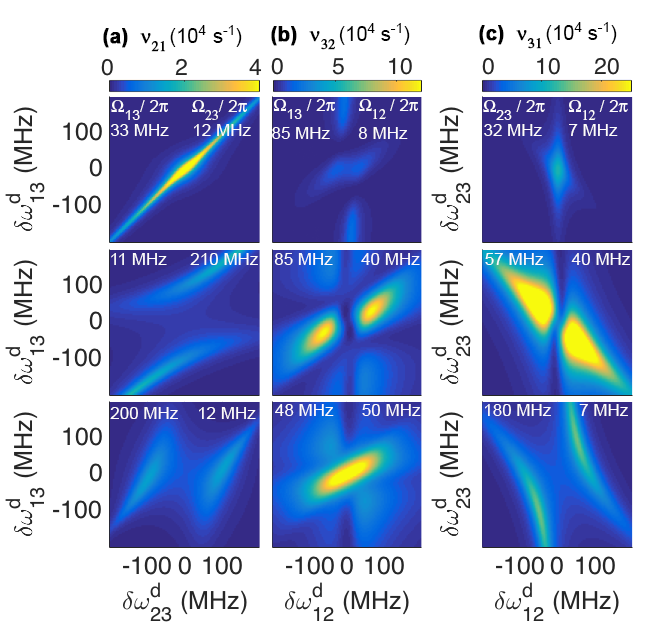
\includegraphics[width=0.85\columnwidth]{fig4-new.png} 
	\caption[Результат численного моделирования когерентной эмиссии, выраженный в единицах фотонного потока ]{Результат численного моделирования когерентной эмиссии, выраженный в единицах фотонного потока $\nu_{em}$ как функция отстроек $\delta\omega^{d}$ двух волн с амплитудами $\Omega_{ij}$ отраженных в подписях поверх панелей.(a) Излучаемый поток фотонов при переходе $\ket{2}\rightarrow \ket{1}$, $\nu^{em}_{21}$ при отмеченных значениях амплитуд $\Omega_{13}$, $\Omega_{23}$. (b) Излучаемый поток фотонов от перехода $\ket{3}\rightarrow \ket{2}$, $\nu^{em}_{32}$, при амплитудах внешних полей $\Omega_{13}$, $\Omega_{12}$. (c): Излучаемый поток фотонов вблизи перехода $\ket{3}\rightarrow \ket{1}$, $\nu^{em}_{31}$, при амплитудах Раби внешних полей $\Omega_{12}$, $\Omega_{23}$.}
	\label{fig:4}
\end{figure}

Заключая, мы продемонстрировали трехволновое смешение в форме когерентного преобразования частоты при помощи одиночного трехуровневого искусственного $\Delta$-атома. Принципиальное отличие нашего устройства от ранее использованных параметрических нелинейных устройствах на основе джозефсоновских переходов состоит в том, что смешение происходит на переходах искусственного атома, находящегося в квантовом режиме, что и определяет свойства рассеянного на атоме излучения. Принципиальным требованием является дипольная разрешенность всех переходов атома, что практически не встречается в природных атомах из-за правил отбора, однако легко реализуется при помощи потокового кубита. Мы надеемся, что полученные результаты найдут применение в создании фотонных сетей и устройств квантовой сверхпроводниковой электроники. 

Следующая глава диссертационной работы посвящена разработке источника одиночных фотонов на базе сверхпроводникового потокового кубита, несимметрично связанного с двумя одномерными полупространствами. Будет показаны результаты многотоновой спектроскопии источника, которая позволяет увидеть большое количество переходов между энергетическими уровнями кубита, а также изучить расщепление Аутлера-Таунса при выборочном драйве переходов. 
 
